% Options for packages loaded elsewhere
\PassOptionsToPackage{unicode}{hyperref}
\PassOptionsToPackage{hyphens}{url}
%
\documentclass[
]{article}
\usepackage{lmodern}
\usepackage{amssymb,amsmath}
\usepackage{ifxetex,ifluatex}
\ifnum 0\ifxetex 1\fi\ifluatex 1\fi=0 % if pdftex
  \usepackage[T1]{fontenc}
  \usepackage[utf8]{inputenc}
  \usepackage{textcomp} % provide euro and other symbols
\else % if luatex or xetex
  \usepackage{unicode-math}
  \defaultfontfeatures{Scale=MatchLowercase}
  \defaultfontfeatures[\rmfamily]{Ligatures=TeX,Scale=1}
\fi
% Use upquote if available, for straight quotes in verbatim environments
\IfFileExists{upquote.sty}{\usepackage{upquote}}{}
\IfFileExists{microtype.sty}{% use microtype if available
  \usepackage[]{microtype}
  \UseMicrotypeSet[protrusion]{basicmath} % disable protrusion for tt fonts
}{}
\makeatletter
\@ifundefined{KOMAClassName}{% if non-KOMA class
  \IfFileExists{parskip.sty}{%
    \usepackage{parskip}
  }{% else
    \setlength{\parindent}{0pt}
    \setlength{\parskip}{6pt plus 2pt minus 1pt}}
}{% if KOMA class
  \KOMAoptions{parskip=half}}
\makeatother
\usepackage{xcolor}
\IfFileExists{xurl.sty}{\usepackage{xurl}}{} % add URL line breaks if available
\IfFileExists{bookmark.sty}{\usepackage{bookmark}}{\usepackage{hyperref}}
\hypersetup{
  pdftitle={Econometrics II - Problem 3},
  pdfauthor={William Radaic Peron},
  hidelinks,
  pdfcreator={LaTeX via pandoc}}
\urlstyle{same} % disable monospaced font for URLs
\usepackage[margin=1in]{geometry}
\usepackage{color}
\usepackage{fancyvrb}
\newcommand{\VerbBar}{|}
\newcommand{\VERB}{\Verb[commandchars=\\\{\}]}
\DefineVerbatimEnvironment{Highlighting}{Verbatim}{commandchars=\\\{\}}
% Add ',fontsize=\small' for more characters per line
\usepackage{framed}
\definecolor{shadecolor}{RGB}{248,248,248}
\newenvironment{Shaded}{\begin{snugshade}}{\end{snugshade}}
\newcommand{\AlertTok}[1]{\textcolor[rgb]{0.94,0.16,0.16}{#1}}
\newcommand{\AnnotationTok}[1]{\textcolor[rgb]{0.56,0.35,0.01}{\textbf{\textit{#1}}}}
\newcommand{\AttributeTok}[1]{\textcolor[rgb]{0.77,0.63,0.00}{#1}}
\newcommand{\BaseNTok}[1]{\textcolor[rgb]{0.00,0.00,0.81}{#1}}
\newcommand{\BuiltInTok}[1]{#1}
\newcommand{\CharTok}[1]{\textcolor[rgb]{0.31,0.60,0.02}{#1}}
\newcommand{\CommentTok}[1]{\textcolor[rgb]{0.56,0.35,0.01}{\textit{#1}}}
\newcommand{\CommentVarTok}[1]{\textcolor[rgb]{0.56,0.35,0.01}{\textbf{\textit{#1}}}}
\newcommand{\ConstantTok}[1]{\textcolor[rgb]{0.00,0.00,0.00}{#1}}
\newcommand{\ControlFlowTok}[1]{\textcolor[rgb]{0.13,0.29,0.53}{\textbf{#1}}}
\newcommand{\DataTypeTok}[1]{\textcolor[rgb]{0.13,0.29,0.53}{#1}}
\newcommand{\DecValTok}[1]{\textcolor[rgb]{0.00,0.00,0.81}{#1}}
\newcommand{\DocumentationTok}[1]{\textcolor[rgb]{0.56,0.35,0.01}{\textbf{\textit{#1}}}}
\newcommand{\ErrorTok}[1]{\textcolor[rgb]{0.64,0.00,0.00}{\textbf{#1}}}
\newcommand{\ExtensionTok}[1]{#1}
\newcommand{\FloatTok}[1]{\textcolor[rgb]{0.00,0.00,0.81}{#1}}
\newcommand{\FunctionTok}[1]{\textcolor[rgb]{0.00,0.00,0.00}{#1}}
\newcommand{\ImportTok}[1]{#1}
\newcommand{\InformationTok}[1]{\textcolor[rgb]{0.56,0.35,0.01}{\textbf{\textit{#1}}}}
\newcommand{\KeywordTok}[1]{\textcolor[rgb]{0.13,0.29,0.53}{\textbf{#1}}}
\newcommand{\NormalTok}[1]{#1}
\newcommand{\OperatorTok}[1]{\textcolor[rgb]{0.81,0.36,0.00}{\textbf{#1}}}
\newcommand{\OtherTok}[1]{\textcolor[rgb]{0.56,0.35,0.01}{#1}}
\newcommand{\PreprocessorTok}[1]{\textcolor[rgb]{0.56,0.35,0.01}{\textit{#1}}}
\newcommand{\RegionMarkerTok}[1]{#1}
\newcommand{\SpecialCharTok}[1]{\textcolor[rgb]{0.00,0.00,0.00}{#1}}
\newcommand{\SpecialStringTok}[1]{\textcolor[rgb]{0.31,0.60,0.02}{#1}}
\newcommand{\StringTok}[1]{\textcolor[rgb]{0.31,0.60,0.02}{#1}}
\newcommand{\VariableTok}[1]{\textcolor[rgb]{0.00,0.00,0.00}{#1}}
\newcommand{\VerbatimStringTok}[1]{\textcolor[rgb]{0.31,0.60,0.02}{#1}}
\newcommand{\WarningTok}[1]{\textcolor[rgb]{0.56,0.35,0.01}{\textbf{\textit{#1}}}}
\usepackage{graphicx,grffile}
\makeatletter
\def\maxwidth{\ifdim\Gin@nat@width>\linewidth\linewidth\else\Gin@nat@width\fi}
\def\maxheight{\ifdim\Gin@nat@height>\textheight\textheight\else\Gin@nat@height\fi}
\makeatother
% Scale images if necessary, so that they will not overflow the page
% margins by default, and it is still possible to overwrite the defaults
% using explicit options in \includegraphics[width, height, ...]{}
\setkeys{Gin}{width=\maxwidth,height=\maxheight,keepaspectratio}
% Set default figure placement to htbp
\makeatletter
\def\fps@figure{htbp}
\makeatother
\setlength{\emergencystretch}{3em} % prevent overfull lines
\providecommand{\tightlist}{%
  \setlength{\itemsep}{0pt}\setlength{\parskip}{0pt}}
\setcounter{secnumdepth}{-\maxdimen} % remove section numbering

\title{Econometrics II - Problem 3}
\author{William Radaic Peron}
\date{\today}

\begin{document}
\maketitle

In this problem, we'll be tackling the issue of \emph{identification} of
an ARMA model. Namely, we will employ the \emph{Box-Jenkins} model
selection strategy, based upon the concept of \emph{parsimony}.

The principle of \emph{parsimony} is inspired on the trade-off between
\emph{fit}, i.e., \(R^2\), and \emph{degrees of freedom}. ``Box and
Jenkins argue that parsimonious models produce better forecasts than
overparametrized models''. (p.~76)

The Box-Jenkins strategy is divided in three main stages:

\begin{itemize}
\item Identification;
\item Estimation;
\item Diagnostic checking.
\end{itemize}

These estimations depend upon two essential conditions (discussed in
earlier problems and lectures): \emph{stationarity} and
\emph{invertibility}. Stationarity, as we have discussed earlier, is
necessary to effectively \emph{employ econometric methods} and to infer
characteristics of a population through a given sample. Enders also
points out that t-statistics and Q-statistics are based upon the
assumption that the data are stationary (p.~77). This implies a
condition on the \emph{AR} process of an ARMA model (roots of
characteristic polynomial outside of unity circle).

Furthermore, the model shall be \emph{invertible} -- i.e., if it can be
represented by a finite or convergent AR model. This implies a condition
on the \emph{MA} process -- i.e., if it can be written as an
AR(\(\infty\)).

We're going to check these conditions intuitively by plotting the ACFs
and PACFs of the time series:

\begin{Shaded}
\begin{Highlighting}[]
\NormalTok{df <-}\StringTok{ }\KeywordTok{data.frame}\NormalTok{(df)}

\NormalTok{pplot <-}\StringTok{ }\KeywordTok{ggplot}\NormalTok{(}\DataTypeTok{data =}\NormalTok{ df, }\KeywordTok{aes}\NormalTok{(}\DataTypeTok{x =}\NormalTok{ t, }\DataTypeTok{y =}\NormalTok{ value)) }\OperatorTok{+}\StringTok{ }\KeywordTok{geom_line}\NormalTok{() }\OperatorTok{+}\StringTok{ }
\StringTok{    }\KeywordTok{ggtitle}\NormalTok{(}\StringTok{"Time series plot"}\NormalTok{) }\OperatorTok{+}\StringTok{ }\KeywordTok{theme_few}\NormalTok{()}
\NormalTok{pplot}
\end{Highlighting}
\end{Shaded}

\begin{center}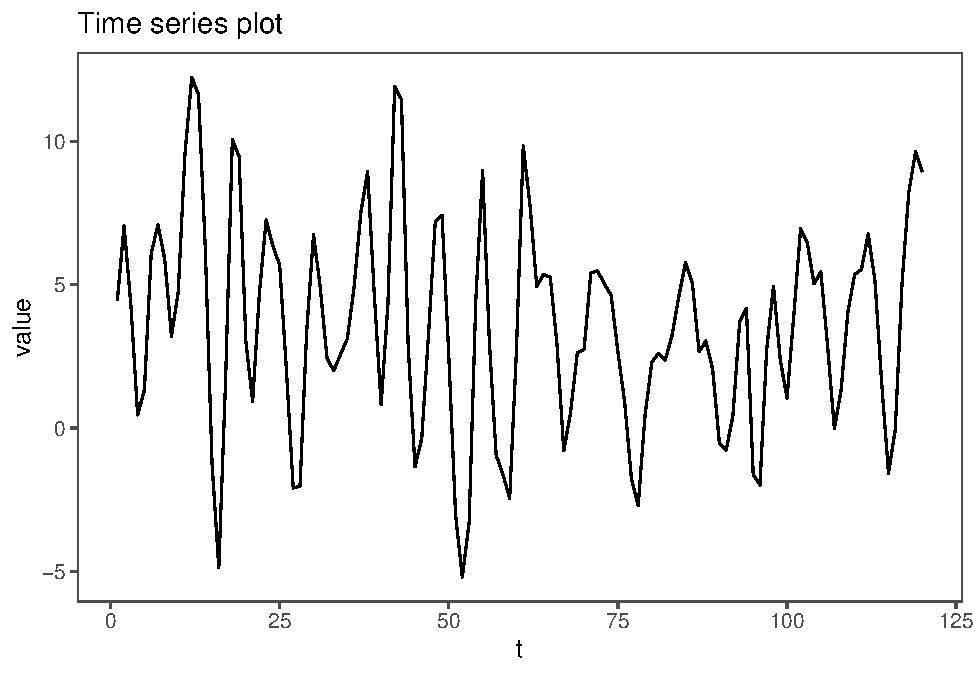
\includegraphics{Econo2_P3_files/figure-latex/plots-1} \end{center}

\begin{Shaded}
\begin{Highlighting}[]
\NormalTok{acf_ts <-}\StringTok{ }\KeywordTok{Acf}\NormalTok{(df}\OperatorTok{$}\NormalTok{value, }\DataTypeTok{lag.max =} \DecValTok{5000}\NormalTok{)}
\end{Highlighting}
\end{Shaded}

\begin{center}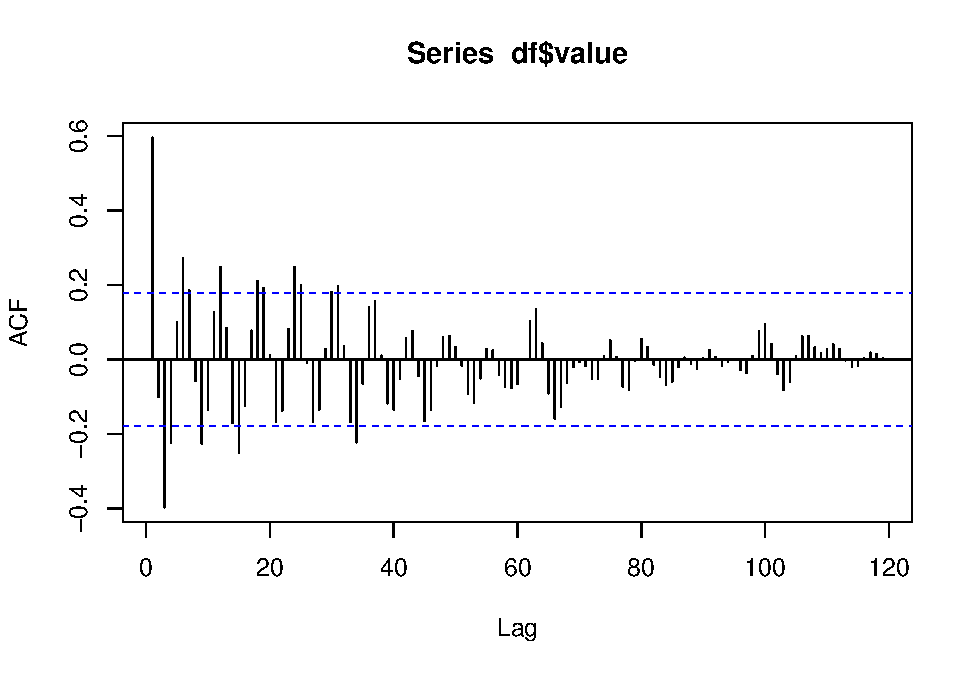
\includegraphics{Econo2_P3_files/figure-latex/plots-2} \end{center}

\begin{Shaded}
\begin{Highlighting}[]
\NormalTok{acf_test_values <-}\StringTok{ }\NormalTok{acf_ts}\OperatorTok{$}\NormalTok{acf}\OperatorTok{/}\KeywordTok{sd}\NormalTok{(acf_ts}\OperatorTok{$}\NormalTok{acf)}

\KeywordTok{head}\NormalTok{(}\KeywordTok{data.frame}\NormalTok{(acf_test_values))}
\end{Highlighting}
\end{Shaded}

\begin{verbatim}
##   acf_test_values
## 1       6.5814152
## 2       3.9180772
## 3      -0.6619326
## 4      -2.6109255
## 5      -1.4713722
## 6       0.6589976
\end{verbatim}

\begin{Shaded}
\begin{Highlighting}[]
\NormalTok{facst <-}\StringTok{ }\KeywordTok{ggAcf}\NormalTok{(df}\OperatorTok{$}\NormalTok{value, }\DataTypeTok{type =} \StringTok{"correlation"}\NormalTok{, }\DataTypeTok{lag.max =} \DecValTok{20}\NormalTok{, }
    \DataTypeTok{plot =}\NormalTok{ T) }\OperatorTok{+}\StringTok{ }\KeywordTok{theme_few}\NormalTok{()}
\NormalTok{faclt <-}\StringTok{ }\KeywordTok{ggAcf}\NormalTok{(df}\OperatorTok{$}\NormalTok{value, }\DataTypeTok{type =} \StringTok{"correlation"}\NormalTok{, }\DataTypeTok{lag.max =} \DecValTok{5000}\NormalTok{, }
    \DataTypeTok{plot =}\NormalTok{ T) }\OperatorTok{+}\StringTok{ }\KeywordTok{theme_few}\NormalTok{()}

\NormalTok{facpst <-}\StringTok{ }\KeywordTok{ggPacf}\NormalTok{(df}\OperatorTok{$}\NormalTok{value, }\DataTypeTok{type =} \StringTok{"correlation"}\NormalTok{, }\DataTypeTok{lag.max =} \DecValTok{100}\NormalTok{, }
    \DataTypeTok{plot =}\NormalTok{ T) }\OperatorTok{+}\StringTok{ }\KeywordTok{theme_few}\NormalTok{()}
\end{Highlighting}
\end{Shaded}

\begin{verbatim}
## Warning: Ignoring unknown parameters: type
\end{verbatim}

\begin{Shaded}
\begin{Highlighting}[]
\NormalTok{facplt <-}\StringTok{ }\KeywordTok{ggPacf}\NormalTok{(df}\OperatorTok{$}\NormalTok{value, }\DataTypeTok{type =} \StringTok{"correlation"}\NormalTok{, }\DataTypeTok{lag.max =} \DecValTok{5000}\NormalTok{, }
    \DataTypeTok{plot =}\NormalTok{ T) }\OperatorTok{+}\StringTok{ }\KeywordTok{theme_few}\NormalTok{()}
\end{Highlighting}
\end{Shaded}

\begin{verbatim}
## Warning: Ignoring unknown parameters: type
\end{verbatim}

\begin{Shaded}
\begin{Highlighting}[]
\NormalTok{facst}
\end{Highlighting}
\end{Shaded}

\begin{center}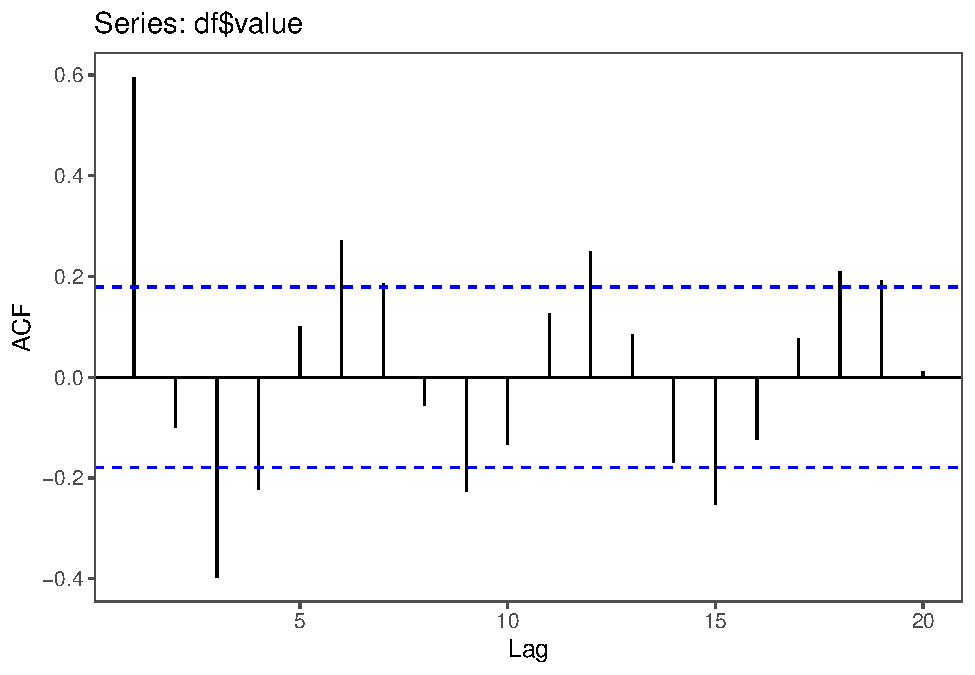
\includegraphics{Econo2_P3_files/figure-latex/plots-3} \end{center}

\begin{Shaded}
\begin{Highlighting}[]
\NormalTok{faclt}
\end{Highlighting}
\end{Shaded}

\begin{center}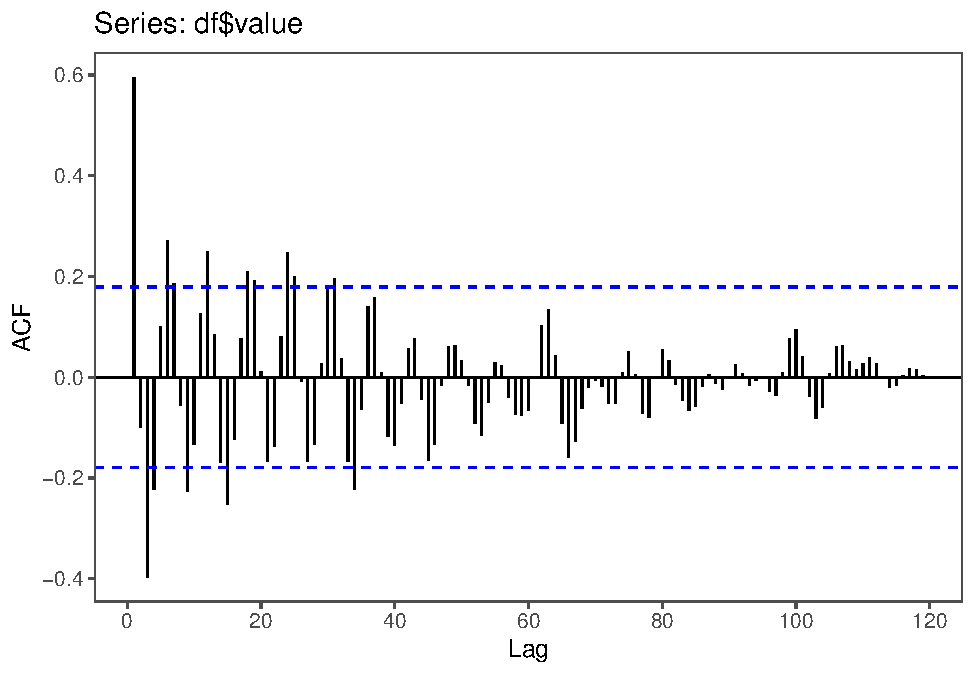
\includegraphics{Econo2_P3_files/figure-latex/plots-4} \end{center}

\begin{Shaded}
\begin{Highlighting}[]
\NormalTok{facpst}
\end{Highlighting}
\end{Shaded}

\begin{center}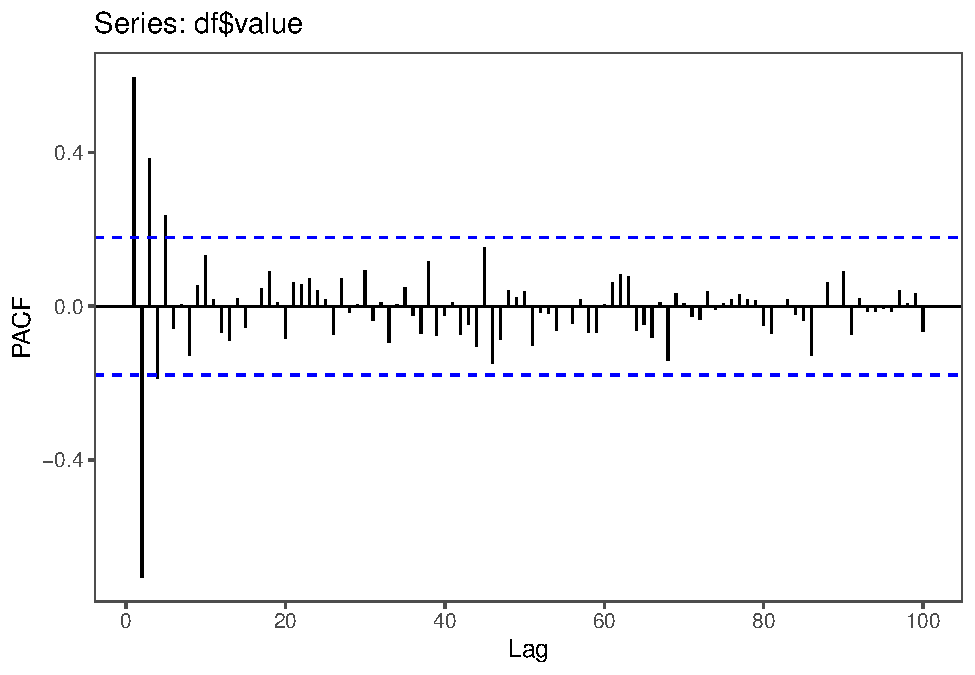
\includegraphics{Econo2_P3_files/figure-latex/plots-5} \end{center}

\begin{Shaded}
\begin{Highlighting}[]
\NormalTok{facplt}
\end{Highlighting}
\end{Shaded}

\begin{center}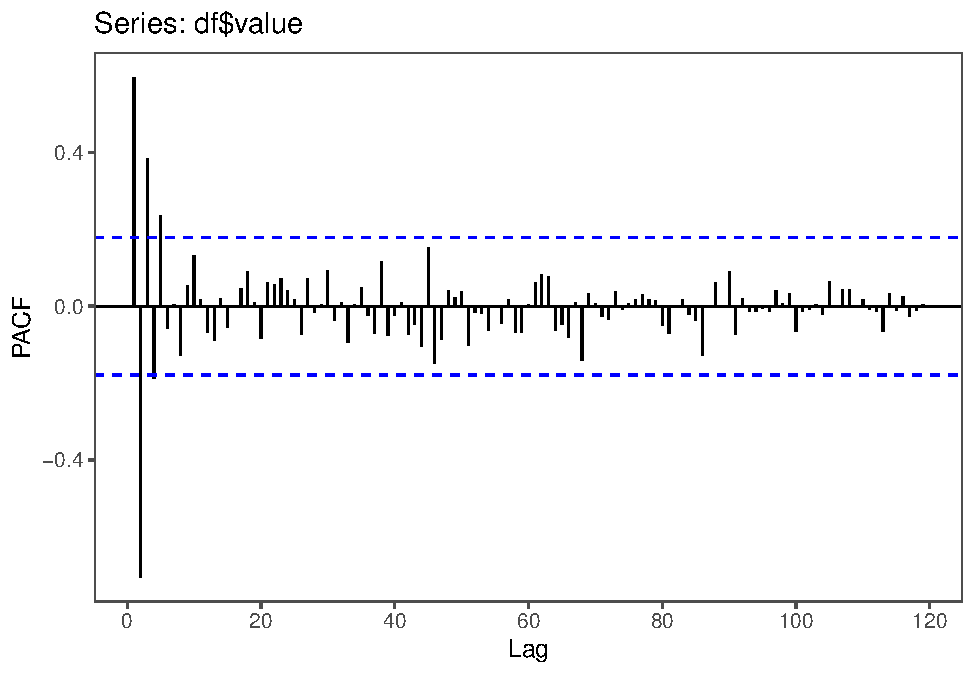
\includegraphics{Econo2_P3_files/figure-latex/plots-6} \end{center}

Aside from usual methods, we'll employ the following criteria:

\begin{itemize}
\item Akaike Information Criterion (AIC). 
$$ AIC = T * ln(SSR) + 2n $$
\item  Schwartz Bayesian Criterion (SBC).
$$ SBC = T * ln(SSR) + n * ln(T) $$
\end{itemize}

\(n\) denotes the number of parameters estimated (an useful metric given
the importance of the degrees of freedom). \(T\) denotes the number of
\emph{usable} observations. Note that, when comparing different models,
it is important to \emph{fix} \(T\) to ensure that the \(AIC\) and
\(SBC\) values are comparable and are capturing only variations in the
actual model and not the effect of changing T.

The objective with these criteria is to \emph{minimize} their values.
``As the fit of the model improves, the AIC and SBC will approach
-\(\infty\).'' (p.~70) \(AIC\) and \(SBC\) have different advantages and
drawbacks: while the former is biased toward overparametrization and
more powerful in small samples, \(SBC\) is consistent and has superior
large sample properties. If both metrics point to the same model, we
should be fairly confident that it is, indeed, the correct
specification.

It is also important to apply hypothesis tests to the estimates of the
population parameters \(\mu, \sigma^2\) and \(\rho_s\) --
\(\bar{y}, \hat{sigma}^2, r_s\), respectively. Worthy of note here is
\(r_s\), which presents the following distributions under the null that
\(y_t\) is stationary with \(\varepsilon_t \sim \mathcal{N}\):
\[ Var(r_s) = T^{-1} \hspace{2em} for \, s = 1\]
\[ Var(r_s) = T^{-1}(1 + 2\sum_{j=1}^{s-1} r_j^2) \hspace{2em} for \, s > 1\]

The Q-statistic is also introduced by Enders in this chapter. It is used
to test whether a group of autocorrelations is significantly different
from zero. \[Q = T\sum_{k=1}^s r_k^2\] Under the null of
\(r_k = 0 \forall k\), Q is asymptotically \(\chi^2\) with s degrees of
freedom. ``Certainly, a white-noise process (in which all
autocorrelations should be zero) would have a Q value of zero''. (p.~68)

An alternative form for \(Q\) is presented by Ljung and Box (1978):
\[ Q = T(T+2) \sum_{k=1}^s \dfrac{r_k^2}{(T-k)} \]

Furthermore, it is also important to check whether the residuals of the
model are actually \emph{white noise}. This can be done via the
Q-statistic, which \emph{should not result in the rejection of the
null}. If that is not the case, the model specified is not the best one
available, as there's still a relevant underlying variable (\(y\) or
\(\varepsilon\)).

Let's now perform the \emph{estimation stage}. This shall be done via
the function \emph{auto.arima} from the package \emph{forecast}.

\begin{Shaded}
\begin{Highlighting}[]
\NormalTok{aa_model <-}\StringTok{ }\KeywordTok{auto.arima}\NormalTok{(df}\OperatorTok{$}\NormalTok{value, }\DataTypeTok{num.cores =} \DecValTok{24}\NormalTok{, }\DataTypeTok{max.d =} \DecValTok{0}\NormalTok{, }\DataTypeTok{max.D =} \DecValTok{0}\NormalTok{, }
    \DataTypeTok{stepwise =}\NormalTok{ F)}

\KeywordTok{summary}\NormalTok{(aa_model)}
\end{Highlighting}
\end{Shaded}

\begin{verbatim}
## Series: df$value 
## ARIMA(2,0,1) with non-zero mean 
## 
## Coefficients:
##          ar1      ar2    ma1    mean
##       0.7524  -0.5545  0.797  3.5305
## s.e.  0.0818   0.0813  0.064  0.3485
## 
## sigma^2 estimated as 3.002:  log likelihood=-235.87
## AIC=481.75   AICc=482.27   BIC=495.68
## 
## Training set error measures:
##                      ME     RMSE      MAE      MPE    MAPE      MASE
## Training set 0.01363546 1.703559 1.426984 5.237664 82.3373 0.5612557
##                     ACF1
## Training set 0.004670695
\end{verbatim}

\begin{Shaded}
\begin{Highlighting}[]
\KeywordTok{print}\NormalTok{(}\StringTok{"t-values: "}\NormalTok{)}
\end{Highlighting}
\end{Shaded}

\begin{verbatim}
## [1] "t-values: "
\end{verbatim}

\begin{Shaded}
\begin{Highlighting}[]
\NormalTok{aa_t <-}\StringTok{ }\KeywordTok{matrix}\NormalTok{(}\OtherTok{NA}\NormalTok{, }\DataTypeTok{nrow =} \DecValTok{4}\NormalTok{)}

\ControlFlowTok{for}\NormalTok{ (i }\ControlFlowTok{in} \KeywordTok{c}\NormalTok{(}\DecValTok{1}\OperatorTok{:}\DecValTok{4}\NormalTok{)) \{}
    
\NormalTok{    aa_t[i] <-}\StringTok{ }\NormalTok{aa_model}\OperatorTok{$}\NormalTok{coef[i]}\OperatorTok{/}\KeywordTok{sqrt}\NormalTok{(aa_model}\OperatorTok{$}\NormalTok{var.coef[i, i])}
    
\NormalTok{\}}

\NormalTok{aa_t <-}\StringTok{ }\KeywordTok{data.frame}\NormalTok{(aa_t)}

\NormalTok{aa_t}
\end{Highlighting}
\end{Shaded}

\begin{verbatim}
##        aa_t
## 1  9.203615
## 2 -6.822352
## 3 12.444488
## 4 10.129782
\end{verbatim}

\begin{Shaded}
\begin{Highlighting}[]
\NormalTok{aa_q <-}\StringTok{ }\KeywordTok{Box.test}\NormalTok{(aa_model}\OperatorTok{$}\NormalTok{residuals, }\DataTypeTok{lag =}\NormalTok{ aa_model}\OperatorTok{$}\NormalTok{arma[}\DecValTok{1}\NormalTok{] }\OperatorTok{+}\StringTok{ }
\StringTok{    }\NormalTok{aa_model}\OperatorTok{$}\NormalTok{arma[}\DecValTok{2}\NormalTok{])}
\NormalTok{aa_q}
\end{Highlighting}
\end{Shaded}

\begin{verbatim}
## 
##  Box-Pierce test
## 
## data:  aa_model$residuals
## X-squared = 0.078351, df = 3, p-value = 0.9943
\end{verbatim}

\begin{Shaded}
\begin{Highlighting}[]
\KeywordTok{ggAcf}\NormalTok{(aa_model}\OperatorTok{$}\NormalTok{residuals, }\DataTypeTok{type =} \StringTok{"correlation"}\NormalTok{, }\DataTypeTok{lag.max =} \DecValTok{20}\NormalTok{, }
    \DataTypeTok{plot =}\NormalTok{ T) }\OperatorTok{+}\StringTok{ }\KeywordTok{theme_few}\NormalTok{()}
\end{Highlighting}
\end{Shaded}

\begin{center}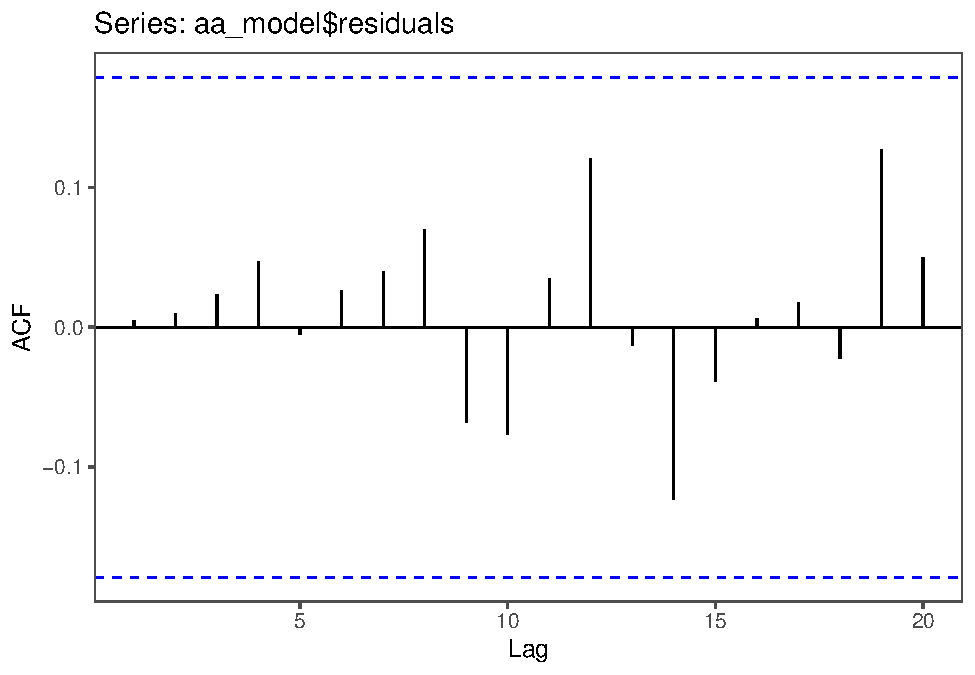
\includegraphics{Econo2_P3_files/figure-latex/estimation autoarima-1} \end{center}

\begin{Shaded}
\begin{Highlighting}[]
\KeywordTok{ggPacf}\NormalTok{(aa_model}\OperatorTok{$}\NormalTok{residuals, }\DataTypeTok{type =} \StringTok{"correlation"}\NormalTok{, }\DataTypeTok{lag.max =} \DecValTok{20}\NormalTok{, }
    \DataTypeTok{plot =}\NormalTok{ T) }\OperatorTok{+}\StringTok{ }\KeywordTok{theme_few}\NormalTok{()}
\end{Highlighting}
\end{Shaded}

\begin{verbatim}
## Warning: Ignoring unknown parameters: type
\end{verbatim}

\begin{center}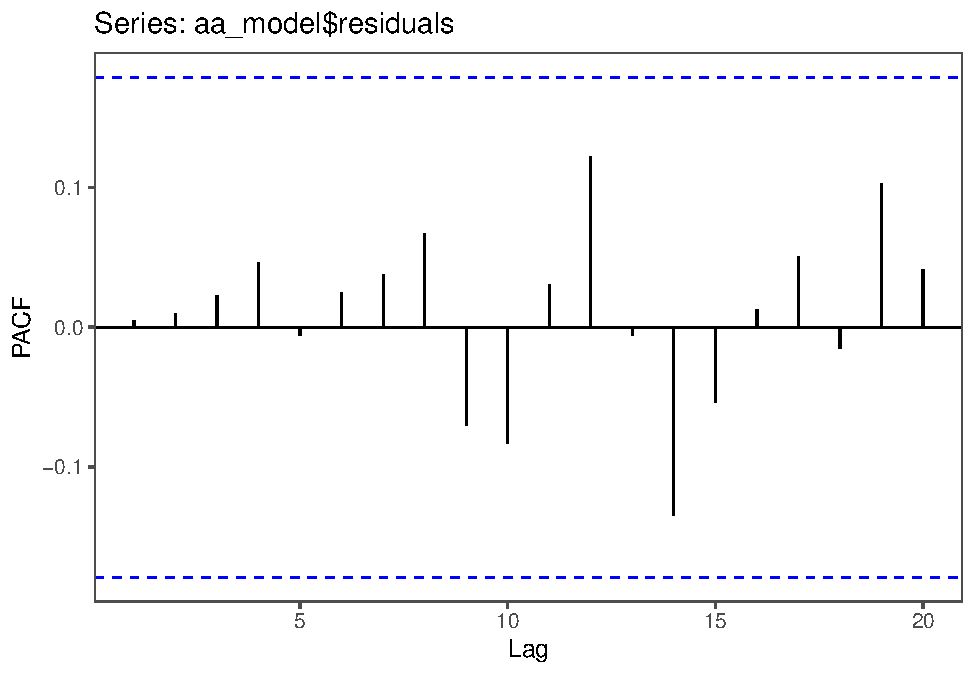
\includegraphics{Econo2_P3_files/figure-latex/estimation autoarima-2} \end{center}

The results of \emph{auto.arima} imply that the best model is an
ARMA(2,1):
\[ y_t = c + \Phi_1 y_{t-1} + \Phi_2 y_{t-2} + \theta_1 \varepsilon_{t-1} + \varepsilon_t, \hspace{1em} \varepsilon_t \sim wn(0, \sigma^2)\]

Furthermore, the Q-statistic \emph{(Box.test)} seems to indicate that
\(\varepsilon_t\) is truly white noise.

Let's now run some different models and compare them against the results
of \emph{auto.arima}. We'll begin with some overspecified model. First,
an ARMA(2,2):
\[ y_t = c + \Phi_1 y_{t-1} + \Phi_2 y_{t-2} + \theta_1 \varepsilon_{t-1} + \theta_2 \varepsilon_{t-2} + \varepsilon_t, \hspace{1em} \varepsilon_t \sim wn(0, \sigma^2)\]

\begin{Shaded}
\begin{Highlighting}[]
\NormalTok{arma22 <-}\StringTok{ }\KeywordTok{Arima}\NormalTok{(df}\OperatorTok{$}\NormalTok{value, }\DataTypeTok{order =} \KeywordTok{c}\NormalTok{(}\DecValTok{2}\NormalTok{, }\DecValTok{0}\NormalTok{, }\DecValTok{2}\NormalTok{))}

\KeywordTok{summary}\NormalTok{(arma22)}
\end{Highlighting}
\end{Shaded}

\begin{verbatim}
## Series: df$value 
## ARIMA(2,0,2) with non-zero mean 
## 
## Coefficients:
##          ar1      ar2     ma1     ma2    mean
##       0.7417  -0.5502  0.8113  0.0149  3.5311
## s.e.  0.1442   0.0950  0.1692  0.1631  0.3514
## 
## sigma^2 estimated as 3.028:  log likelihood=-235.87
## AIC=483.74   AICc=484.48   BIC=500.46
## 
## Training set error measures:
##                      ME     RMSE      MAE      MPE     MAPE      MASE
## Training set 0.01360342 1.703508 1.426237 4.791703 81.74486 0.5609619
##                     ACF1
## Training set 0.001161589
\end{verbatim}

\begin{Shaded}
\begin{Highlighting}[]
\NormalTok{arma22_t <-}\StringTok{ }\KeywordTok{matrix}\NormalTok{(}\OtherTok{NA}\NormalTok{, }\DataTypeTok{nrow =} \DecValTok{5}\NormalTok{)}

\ControlFlowTok{for}\NormalTok{ (i }\ControlFlowTok{in} \KeywordTok{c}\NormalTok{(}\DecValTok{1}\OperatorTok{:}\DecValTok{5}\NormalTok{)) \{}
    
\NormalTok{    arma22_t[i] <-}\StringTok{ }\NormalTok{arma22}\OperatorTok{$}\NormalTok{coef[i]}\OperatorTok{/}\KeywordTok{sqrt}\NormalTok{(arma22}\OperatorTok{$}\NormalTok{var.coef[i, i])}
    
\NormalTok{\}}

\NormalTok{arma22_t <-}\StringTok{ }\KeywordTok{data.frame}\NormalTok{(arma22_t)}

\NormalTok{arma22_t}
\end{Highlighting}
\end{Shaded}

\begin{verbatim}
##      arma22_t
## 1  5.14206433
## 2 -5.78853038
## 3  4.79577309
## 4  0.09134106
## 5 10.04968297
\end{verbatim}

\begin{Shaded}
\begin{Highlighting}[]
\NormalTok{arma22_q <-}\StringTok{ }\KeywordTok{Box.test}\NormalTok{(arma22}\OperatorTok{$}\NormalTok{residuals, }\DataTypeTok{lag =}\NormalTok{ arma22}\OperatorTok{$}\NormalTok{arma[}\DecValTok{1}\NormalTok{] }\OperatorTok{+}\StringTok{ }
\StringTok{    }\NormalTok{arma22}\OperatorTok{$}\NormalTok{arma[}\DecValTok{2}\NormalTok{])}
\NormalTok{arma22_q}
\end{Highlighting}
\end{Shaded}

\begin{verbatim}
## 
##  Box-Pierce test
## 
## data:  arma22$residuals
## X-squared = 0.26458, df = 4, p-value = 0.992
\end{verbatim}

The t-value of \(ma2\) is not able to reject the null hypothesis.
Furthermore, the Q-statistic \emph{(Box.test)} seems to indicate that
\(\varepsilon_t\) is truly white noise.

Now, an ARMA(3,1):
\[ y_t = c + \Phi_1 y_{t-1} + \Phi_2 y_{t-2} + \Phi_3 y_{t-3} + \theta_1 \varepsilon_{t-1} + \varepsilon_t, \hspace{1em} \varepsilon_t \sim wn(0, \sigma^2)\]

\begin{Shaded}
\begin{Highlighting}[]
\NormalTok{arma31 <-}\StringTok{ }\KeywordTok{Arima}\NormalTok{(df}\OperatorTok{$}\NormalTok{value, }\DataTypeTok{order =} \KeywordTok{c}\NormalTok{(}\DecValTok{3}\NormalTok{, }\DecValTok{0}\NormalTok{, }\DecValTok{1}\NormalTok{))}

\KeywordTok{summary}\NormalTok{(arma31)}
\end{Highlighting}
\end{Shaded}

\begin{verbatim}
## Series: df$value 
## ARIMA(3,0,1) with non-zero mean 
## 
## Coefficients:
##          ar1     ar2     ar3     ma1    mean
##       0.7610  -0.565  0.0112  0.7923  3.5312
## s.e.  0.1215   0.137  0.1174  0.0825  0.3516
## 
## sigma^2 estimated as 3.028:  log likelihood=-235.87
## AIC=483.74   AICc=484.48   BIC=500.46
## 
## Training set error measures:
##                      ME     RMSE      MAE      MPE     MAPE      MASE
## Training set 0.01359734 1.703504 1.426202 4.779284 81.71699 0.5609482
##                      ACF1
## Training set 0.0008885573
\end{verbatim}

\begin{Shaded}
\begin{Highlighting}[]
\NormalTok{arma31_t <-}\StringTok{ }\KeywordTok{matrix}\NormalTok{(}\OtherTok{NA}\NormalTok{, }\DataTypeTok{nrow =} \DecValTok{5}\NormalTok{)}

\ControlFlowTok{for}\NormalTok{ (i }\ControlFlowTok{in} \KeywordTok{c}\NormalTok{(}\DecValTok{1}\OperatorTok{:}\DecValTok{5}\NormalTok{)) \{}
    
\NormalTok{    arma31_t[i] <-}\StringTok{ }\NormalTok{arma31}\OperatorTok{$}\NormalTok{coef[i]}\OperatorTok{/}\KeywordTok{sqrt}\NormalTok{(arma31}\OperatorTok{$}\NormalTok{var.coef[i, i])}
    
\NormalTok{\}}

\NormalTok{arma31_t <-}\StringTok{ }\KeywordTok{data.frame}\NormalTok{(arma31_t)}

\NormalTok{arma31_t}
\end{Highlighting}
\end{Shaded}

\begin{verbatim}
##      arma31_t
## 1  6.26539086
## 2 -4.12346904
## 3  0.09501299
## 4  9.59788435
## 5 10.04172094
\end{verbatim}

\begin{Shaded}
\begin{Highlighting}[]
\NormalTok{arma31_q <-}\StringTok{ }\KeywordTok{Box.test}\NormalTok{(arma31}\OperatorTok{$}\NormalTok{residuals, }\DataTypeTok{lag =}\NormalTok{ arma31}\OperatorTok{$}\NormalTok{arma[}\DecValTok{1}\NormalTok{] }\OperatorTok{+}\StringTok{ }
\StringTok{    }\NormalTok{arma31}\OperatorTok{$}\NormalTok{arma[}\DecValTok{2}\NormalTok{])}
\NormalTok{arma31_q}
\end{Highlighting}
\end{Shaded}

\begin{verbatim}
## 
##  Box-Pierce test
## 
## data:  arma31$residuals
## X-squared = 0.25911, df = 4, p-value = 0.9923
\end{verbatim}

The t-value of \(ar3\) is not able to reject the null hypothesis.
Furthermore, the Q-statistic \emph{(Box.test)} seems to indicate that
\(\varepsilon_t\) is truly white noise.

Now, let's try some \emph{underspecified models}. Beginning with an
ARMA(2,0):
\[ y_t = c + \Phi_1 y_{t-1} + \Phi_2 y_{t-2} + \varepsilon_t, \hspace{1em} \varepsilon_t \sim wn(0, \sigma^2)\]

\begin{Shaded}
\begin{Highlighting}[]
\NormalTok{arma20 <-}\StringTok{ }\KeywordTok{Arima}\NormalTok{(df}\OperatorTok{$}\NormalTok{value, }\DataTypeTok{order =} \KeywordTok{c}\NormalTok{(}\DecValTok{2}\NormalTok{, }\DecValTok{0}\NormalTok{, }\DecValTok{0}\NormalTok{))}

\KeywordTok{summary}\NormalTok{(arma20)}
\end{Highlighting}
\end{Shaded}

\begin{verbatim}
## Series: df$value 
## ARIMA(2,0,0) with non-zero mean 
## 
## Coefficients:
##          ar1      ar2    mean
##       1.0226  -0.7153  3.5194
## s.e.  0.0634   0.0635  0.2694
## 
## sigma^2 estimated as 4.24:  log likelihood=-256.37
## AIC=520.74   AICc=521.09   BIC=531.89
## 
## Training set error measures:
##                      ME     RMSE      MAE      MPE     MAPE      MASE      ACF1
## Training set 0.01106086 2.033314 1.630805 73.16585 128.4039 0.6414218 0.2915253
\end{verbatim}

\begin{Shaded}
\begin{Highlighting}[]
\NormalTok{arma20_t <-}\StringTok{ }\KeywordTok{matrix}\NormalTok{(}\OtherTok{NA}\NormalTok{, }\DataTypeTok{nrow =} \DecValTok{3}\NormalTok{)}

\ControlFlowTok{for}\NormalTok{ (i }\ControlFlowTok{in} \KeywordTok{c}\NormalTok{(}\DecValTok{1}\OperatorTok{:}\DecValTok{3}\NormalTok{)) \{}
    
\NormalTok{    arma20_t[i] <-}\StringTok{ }\NormalTok{arma20}\OperatorTok{$}\NormalTok{coef[i]}\OperatorTok{/}\KeywordTok{sqrt}\NormalTok{(arma20}\OperatorTok{$}\NormalTok{var.coef[i, i])}
    
\NormalTok{\}}

\NormalTok{arma20_t <-}\StringTok{ }\KeywordTok{data.frame}\NormalTok{(arma20_t)}

\NormalTok{arma20_t}
\end{Highlighting}
\end{Shaded}

\begin{verbatim}
##    arma20_t
## 1  16.12226
## 2 -11.26848
## 3  13.06561
\end{verbatim}

\begin{Shaded}
\begin{Highlighting}[]
\NormalTok{arma20_q <-}\StringTok{ }\KeywordTok{Box.test}\NormalTok{(arma20}\OperatorTok{$}\NormalTok{residuals, }\DataTypeTok{lag =}\NormalTok{ arma20}\OperatorTok{$}\NormalTok{arma[}\DecValTok{1}\NormalTok{] }\OperatorTok{+}\StringTok{ }
\StringTok{    }\NormalTok{arma20}\OperatorTok{$}\NormalTok{arma[}\DecValTok{2}\NormalTok{])}
\NormalTok{arma20_q}
\end{Highlighting}
\end{Shaded}

\begin{verbatim}
## 
##  Box-Pierce test
## 
## data:  arma20$residuals
## X-squared = 13.728, df = 2, p-value = 0.001045
\end{verbatim}

The Q-statistic indicates that there is an ommited variable -- namely,
\(\varepsilon_{t-1}\) that we have just excluded from the model.

Now, an ARMA(1,1):
\[ y_t = c + \Phi_1 y_{t-1} +  + \theta_1 \varepsilon_{t-1} + \varepsilon_t, \hspace{1em} \varepsilon_t \sim wn(0, \sigma^2)\]

\begin{Shaded}
\begin{Highlighting}[]
\NormalTok{arma11 <-}\StringTok{ }\KeywordTok{Arima}\NormalTok{(df}\OperatorTok{$}\NormalTok{value, }\DataTypeTok{order =} \KeywordTok{c}\NormalTok{(}\DecValTok{1}\NormalTok{, }\DecValTok{0}\NormalTok{, }\DecValTok{1}\NormalTok{))}

\KeywordTok{summary}\NormalTok{(arma11)}
\end{Highlighting}
\end{Shaded}

\begin{verbatim}
## Series: df$value 
## ARIMA(1,0,1) with non-zero mean 
## 
## Coefficients:
##          ar1     ma1    mean
##       0.4476  0.9244  3.6027
## s.e.  0.0831  0.0323  0.6234
## 
## sigma^2 estimated as 4.026:  log likelihood=-253.74
## AIC=515.48   AICc=515.82   BIC=526.63
## 
## Training set error measures:
##                       ME     RMSE      MAE      MPE     MAPE      MASE
## Training set 0.006283661 1.981184 1.621537 51.07775 142.3988 0.6377767
##                   ACF1
## Training set 0.2028683
\end{verbatim}

\begin{Shaded}
\begin{Highlighting}[]
\NormalTok{arma11_t <-}\StringTok{ }\KeywordTok{matrix}\NormalTok{(}\OtherTok{NA}\NormalTok{, }\DataTypeTok{nrow =} \DecValTok{3}\NormalTok{)}

\ControlFlowTok{for}\NormalTok{ (i }\ControlFlowTok{in} \KeywordTok{c}\NormalTok{(}\DecValTok{1}\OperatorTok{:}\DecValTok{3}\NormalTok{)) \{}
    
\NormalTok{    arma11_t[i] <-}\StringTok{ }\NormalTok{arma11}\OperatorTok{$}\NormalTok{coef[i]}\OperatorTok{/}\KeywordTok{sqrt}\NormalTok{(arma11}\OperatorTok{$}\NormalTok{var.coef[i, i])}
    
\NormalTok{\}}

\NormalTok{arma11_t <-}\StringTok{ }\KeywordTok{data.frame}\NormalTok{(arma11_t)}

\NormalTok{arma11_t}
\end{Highlighting}
\end{Shaded}

\begin{verbatim}
##    arma11_t
## 1  5.387948
## 2 28.624391
## 3  5.779126
\end{verbatim}

\begin{Shaded}
\begin{Highlighting}[]
\NormalTok{arma11_q <-}\StringTok{ }\KeywordTok{Box.test}\NormalTok{(arma11}\OperatorTok{$}\NormalTok{residuals, }\DataTypeTok{lag =}\NormalTok{ arma11}\OperatorTok{$}\NormalTok{arma[}\DecValTok{1}\NormalTok{] }\OperatorTok{+}\StringTok{ }
\StringTok{    }\NormalTok{arma11}\OperatorTok{$}\NormalTok{arma[}\DecValTok{2}\NormalTok{])}
\NormalTok{arma11_q}
\end{Highlighting}
\end{Shaded}

\begin{verbatim}
## 
##  Box-Pierce test
## 
## data:  arma11$residuals
## X-squared = 12.668, df = 2, p-value = 0.001775
\end{verbatim}

Again, the Q-statistic indicates that there is an ommited variable --
namely, \(y_{t-1}\) that we have just excluded from the model.

Finally, let's compare the \(AIC\) and \(BIC\) values for all these
models.

\begin{Shaded}
\begin{Highlighting}[]
\NormalTok{criteria <-}\StringTok{ }\KeywordTok{matrix}\NormalTok{(}\OtherTok{NA}\NormalTok{, }\DataTypeTok{nrow =} \DecValTok{5}\NormalTok{, }\DataTypeTok{ncol =} \DecValTok{3}\NormalTok{)}

\NormalTok{aa_criteria <-}\StringTok{ }\KeywordTok{data.frame}\NormalTok{(}\StringTok{"ARMA(2,1)*"}\NormalTok{, aa_model}\OperatorTok{$}\NormalTok{aic, aa_model}\OperatorTok{$}\NormalTok{bic)}

\KeywordTok{names}\NormalTok{(aa_criteria) <-}\StringTok{ }\KeywordTok{c}\NormalTok{(}\StringTok{"Model"}\NormalTok{, }\StringTok{"AIC"}\NormalTok{, }\StringTok{"BIC"}\NormalTok{)}

\NormalTok{arma22_criteria <-}\StringTok{ }\KeywordTok{data.frame}\NormalTok{(}\StringTok{"ARMA(2,2)"}\NormalTok{, arma22}\OperatorTok{$}\NormalTok{aic, arma22}\OperatorTok{$}\NormalTok{bic)}

\KeywordTok{names}\NormalTok{(arma22_criteria) <-}\StringTok{ }\KeywordTok{c}\NormalTok{(}\StringTok{"Model"}\NormalTok{, }\StringTok{"AIC"}\NormalTok{, }\StringTok{"BIC"}\NormalTok{)}

\NormalTok{arma31_criteria <-}\StringTok{ }\KeywordTok{data.frame}\NormalTok{(}\StringTok{"ARMA(3,1)"}\NormalTok{, arma31}\OperatorTok{$}\NormalTok{aic, arma31}\OperatorTok{$}\NormalTok{bic)}

\KeywordTok{names}\NormalTok{(arma31_criteria) <-}\StringTok{ }\KeywordTok{c}\NormalTok{(}\StringTok{"Model"}\NormalTok{, }\StringTok{"AIC"}\NormalTok{, }\StringTok{"BIC"}\NormalTok{)}

\NormalTok{arma20_criteria <-}\StringTok{ }\KeywordTok{data.frame}\NormalTok{(}\StringTok{"ARMA(2,0)"}\NormalTok{, arma20}\OperatorTok{$}\NormalTok{aic, arma20}\OperatorTok{$}\NormalTok{bic)}

\KeywordTok{names}\NormalTok{(arma20_criteria) <-}\StringTok{ }\KeywordTok{c}\NormalTok{(}\StringTok{"Model"}\NormalTok{, }\StringTok{"AIC"}\NormalTok{, }\StringTok{"BIC"}\NormalTok{)}

\NormalTok{arma11_criteria <-}\StringTok{ }\KeywordTok{data.frame}\NormalTok{(}\StringTok{"ARMA(1,1)"}\NormalTok{, arma11}\OperatorTok{$}\NormalTok{aic, arma11}\OperatorTok{$}\NormalTok{bic)}

\KeywordTok{names}\NormalTok{(arma11_criteria) <-}\StringTok{ }\KeywordTok{c}\NormalTok{(}\StringTok{"Model"}\NormalTok{, }\StringTok{"AIC"}\NormalTok{, }\StringTok{"BIC"}\NormalTok{)}


\NormalTok{criteria <-}\StringTok{ }\KeywordTok{rbind.data.frame}\NormalTok{(aa_criteria, arma22_criteria, arma31_criteria, }
\NormalTok{    arma20_criteria, arma11_criteria)}

\NormalTok{criteria}
\end{Highlighting}
\end{Shaded}

\begin{verbatim}
##        Model      AIC      BIC
## 1 ARMA(2,1)* 481.7460 495.6834
## 2  ARMA(2,2) 483.7376 500.4625
## 3  ARMA(3,1) 483.7369 500.4619
## 4  ARMA(2,0) 520.7381 531.8880
## 5  ARMA(1,1) 515.4753 526.6253
\end{verbatim}

As we can clearly see, the model chosen by \emph{auto.arima} is the
optimal choice according both to AIC and BIC.

\end{document}
